\documentclass[12pt]{article}

\PassOptionsToPackage{backend=biber, style=numeric, sorting=none}{biblatex}

\usepackage{paper,math}

\usepackage[T2A]{fontenc}
\usepackage[utf8]{inputenc}
\usepackage[russian,english]{babel}
\usepackage{csquotes}

% For algorithm representation
\usepackage{algorithm}
\usepackage{algpseudocode}

% For pretty tables
\usepackage{booktabs}
\usepackage{caption}

% Add the local reference file
\addbibresource{refs.bib}

\hfuzz=30pt % Suppresses warnings for lines up to 30pt too wide
\sloppy

\title{Моделирование производительности кластера Kubernetes учитывающее состояния системы и характер смешанной нагрузки}
\author{
  Мельничук Михаил, Владимир Анатольевич Богатырёв\\ {\itshape\large Университет ИТМО}\\
}
\date{\today}

\booltrue{INCLUDECOMMENTS}
\newcommand{\kyle}[1]{\coauthorComment[Kyle]{#1}}

\graphicspath{{Melnichuk_Figs/}}
\captionsetup[figure]{name=Fig.}

\begin{document}

% ##################################################################################################
% Title Page
\maketitle
\begin{abstract}
  В представленной работе проведён анализ производительности кластера контейнерной виртуализации Kubernetes с учётом смешанного характера рабочей нагрузки, которая включает как вычислительно интенсивные запросы, так и запросы, связанные с операциями ввода-вывода. Предложена и верифицирована аналитическая модель системы массового обслуживания, в которой эффективная интенсивность обслуживания является функцией трёх параметров: числа контейнеров, доли вычислительных запросов и текущего числа заявок в системе. Для практической оценки указанной зависимости разработан метод калибровки интенсивности обслуживания по эмпирическим данным, полученным на двухузловом кластере Kubernetes с выделенным аппаратным обеспечением. С помощью полиномиальной регрессии второй степени построена модель, предсказывающая значение обслуживания каждого пода для произвольных комбинаций параметров. Проведено сравнение предложенного подхода с моделью не учитывающей состояние системы, которое демонстрирует, что учёт числа заявок в системе позволяет повысить точность прогнозирования времени отклика. Корректность аналитического решения подтверждена имитационной моделью на SimPy, прошедшей верификацию cо средней абсолютной процентной ошибкой (MAPE) 0,50\% ($\pm$0,49\%--0,51\%). Полученные результаты могут служить основой для принятия решений при автоматическом масштабировании контейнерных кластеров.
\end{abstract}

% ==================================================================================================
% 1. INTRODUCTION
% ==================================================================================================
\section{Введение}
\label{sec:introduction}

Kubernetes в последние годы стал фактическим стандартом для развёртывания распределённых приложений, как в облачных, так и в периферийных средах \cite{pahl2017cloud}. Гибкость, автоматизация и масштабируемость встроенны в технологию облегчая работу инженеров. Вот только эффективно ею пользоваться без глубокого понимания факторов производительности попросту невозможно. Особенно остро это проявляется в задачах автомасштабирования, планирования ресурсов и обеспечения качества обслуживания. Каждая из них опирается на одно и то же: умение прогнозировать время отклика при разных уровнях нагрузки и разных конфигурациях кластера \cite{al2017elasticity}. Без точной модели производительности, невозможно принять обоснованное решение, когда рабочая нагрузка меняется динамически.

Подходов к моделированию производительности контейнерных систем в литературе накопилось немало. Классическая теория массового обслуживания по-прежнему остаётся фундаментальным инструментом, и к Kubernetes её применяют всё активнее. Возьмём, к примеру, работу \cite{pan2024performance}: там проанализированы три алгоритма планирования заданий через одноканальную M/M/1 и многосерверную M/M/s модели. Авторами было выявлено что многоканальная M/M/s даёт лучшие показатели. Однако этот подход, как и большинство классических моделей \cite{kleinrock1974queueing}, предполагает постоянную интенсивность обслуживания. А в реальной системе накладные расходы сети, балансировщика и планировщика Kubernetes существенно варьируются в зависимости от загрузки \cite{koukis2024performance, luo2021characterizing, shahrad2020serverless}. Разрыв между теоретическими допущениями и практикой, здесь вполне ощутимый.

Есть и аналитические модели. Здесь интенсивность обслуживания зависит от числа контейнеров и текущего числа заявок. В \cite{van2024evaluation} предложен комплексный подход включающий аналитическую модель, имитацию на SimPy и натурные эксперименты на Kubernetes. Интенсивность обслуживания там привязана к состоянию системы, а влияние числа контейнеров на временные характеристики исследовано достаточно подробно. Данная работа пожалуй, наиболее близкий аналог нашего исследования. Но вот смешанная нагрузка, определяемая долей вычислительных запросов, в ней не учтена, а это серьёзно ограничивает применимость для гетерогенных потоков. Близкие по духу решения есть в \cite{berner2025improved} и \cite{cai2021inverse}, данные модели с переменной интенсивностью для управления очередями и эластичного предоставления контейнеров. Однако, акцент этих работ сделан на управляющие воздействия, а не на калибровку по эмпирическим данным.

Отдельную нишу занимают имитационное моделирование и специализированные инструменты симуляции. Платформа KubeTwin \cite{Santos2026KubeTwin2D}, создаёт цифровые двойники кластеров для безопасного экспериментирования с политиками планирования. MicroViSim \cite{lin2025microvisim} ориентирован на визуализацию узких мест. Существует также модульный симулятор рабочей нагрузки для оценки политик планирования на основе машинного обучения \cite{touloupoumodular}. Проблема в том, что аналитических выражений для времени отклика такие решения, как правило, не дают, а вычислительных ресурсов на симуляции требуют немало.

Помимо этого, активно развиваются методы на основе машинного обучения. Среди них Mixture Density Networks для характеризации распределения времени ответа \cite{manca2023characterization}, модели на обобщённых стохастических сетях Петри для оптимизации производительности и энергопотребления \cite{fe2025energy}. В последнее время появились подходы с графовыми нейронными сетями \cite{richart2025lq} и с обучением с подкреплением для оптимизации развёртывания микросервисов \cite{peng2024delay}. Их гибкость высокая, но к сожалению интерпретируемость низкая, не говоря о количестве размеченных данных для их обучения. Работа \cite{jindal2019performance} заслуживает отдельного упоминания, там пропускная способность микросервисов определяется через изолированное нагрузочное тестирование с регрессионным моделированием. Это лишний раз подчёркивает, насколько важна эмпирическая калибровка для точного прогноза.

Анализ приведённых работ обнажает вполне конкретный пробел. На сегодняшний день нет аналитической модели, которая одновременно учитывала бы зависимость интенсивности обслуживания от числа заявок в системе, отражала влияние смешанной нагрузки и калибровалась по эмпирическим данным с учётом всех накладных расходов Kubernetes. Восполнить этот пробел и есть цель настоящего исследования.

В этой работе мы предлагаем модель, где интенсивность обслуживания зависит сразу от трёх параметров: числа контейнеров, доли вычислительных запросов и текущего числа заявок. Как её оценить на практике? Мы разработали метод калибровки по эмпирическим замерам полного времени обслуживания — причём учтены все скрытые, трудноуловимые задержки. Для предсказания интенсивности при любых сочетаниях параметров взяли полиномиальную регрессию второй степени. Верификацию провели двояко: на экспериментальных данных двухузлового кластера Kubernetes и через имитацию в SimPy. Результат сравнения с классической моделью, игнорирующей состояние системы, однозначен: учёт текущего состояния заметно повышает точность прогноза времени отклика.

Новизна исследования заключается в следующем. Разработана аналитическая модель с интенсивностью обслуживания, зависящей от числа контейнеров, доли вычислительных запросов и текущего числа заявок. Предложен метод калибровки этой интенсивности по эмпирическим данным, позволяющий учесть все накладные расходы Kubernetes. Построена регрессионная модель для предсказания интенсивности, и продемонстрировано её преимущество перед классическим подходом без учёта состояния системы. И наконец, разработана и верифицирована имитационная модель, подтверждающая корректность аналитического решения.

Статья организована так. Раздел~2 описывает экспериментальный стенд, математическую модель, процедуру калибровки, регрессионную модель и постановку имитационного эксперимента. В разделе~3 представлены результаты численного моделирования: анализ устойчивости вычислений, сравнение регрессионных моделей, верификация имитации. Раздел~4 посвящён обсуждению результатов, их ограничений и практической значимости. Основные выводы и направления будущих исследований собраны в разделе~5.

% ==================================================================================================
% 2. MATERIALS AND METHODS
% ==================================================================================================
\section{Материалы и методы}
\label{sec:methods}

\subsection{Экспериментальная установка}

В работе \cite{мельничук2026анализ} описана платформа оркестрации контейнеров Kubernetes. Архитектура этого стенда показана на рис. \ref{fig:Experimental_Setup}, представляет собой физический сервер с гипервизором Proxmox, на котором развёрнут двухузловой кластер Kubernetes (управляющий и рабочий узлы). Входящий поток запросов предполагается пуассоновским с интенсивностью $\lambda$. Балансировщик нагрузки распределяет запросы между рабочими контейнерами по алгоритму Round Robin. Такая конфигурация обеспечивает изоляцию ресурсов и воспроизводимость измерений.

Микросервис обробатывающий запросы реализован как контейнер Docker без сохранения состояния (stateless). Каждый контейнер поддерживает обработку запросов двух типов: (i) ресурсоёмкие вычислительные задачи и (ii) операции ввода-вывода. Горизонтальное масштабирование выполняется запуском $n$ идентичных реплик (подов) этого контейнера. В модели они рассматриваются как $n$ однородных серверов, в то время как планировщик Kubernetes распределяет поды по узлам кластера.

\begin{figure}[!htbp]
  \centering
  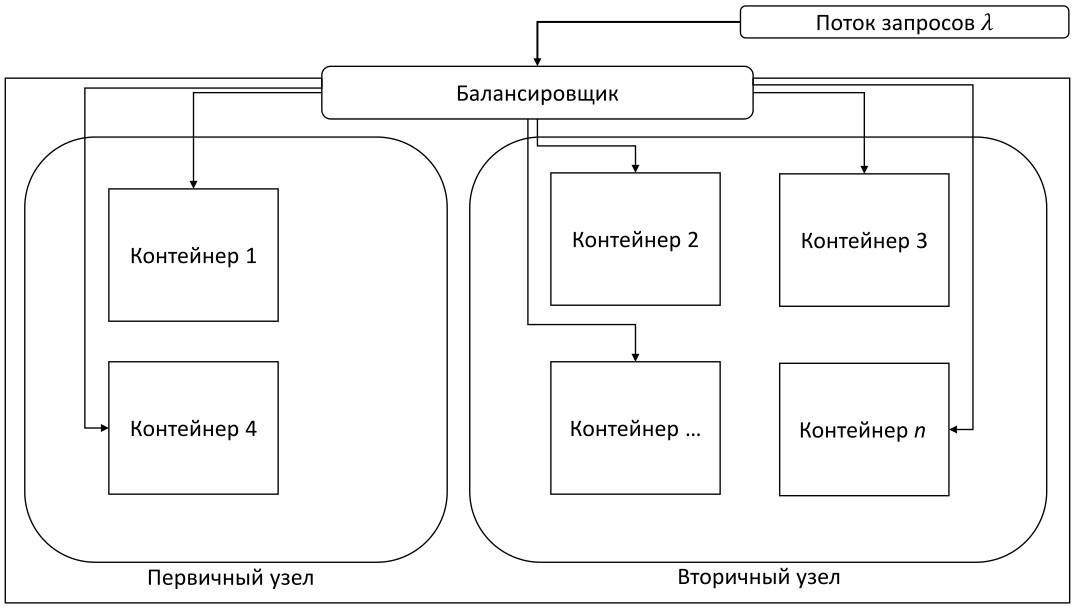
\includegraphics[height=5cm]{Experimental_Setup.jpeg}
  \caption{Схема эксперимента: двухузловой кластер Kubernetes, развёрнутый на выделенном сервере Proxmox. В состав кластера входит балансировщик нагрузки, обеспечивающий распределение входящего потока запросов, а также $n$ контейнеров обрабатывающих пользовательские запросы.}
  \label{fig:Experimental_Setup}
\end{figure}


\subsection{Модель СМО с интенсивностью обслуживания зависимой состояния системы}

Нагрузка на систему формировалась смешанным потоком запросов. Ключевой независимой переменной в настоящем исследовании являлся параметр $\alpha$ (альфа), определяющий долю запросов, требующих интенсивных вычислений центрального процессора (ЦП). Соответственно, доля запросов, связанных с операциями ввода-вывода составляла $(1-\alpha)$.

Предполагается, что входящий поток подчиняется пуассоновскому закону распределения с интенсивностью $\lambda$, а интенсивность обслуживания $\mu(n,\alpha,i)$ представляет собой функцию зависящей от числа контейнеров $n$, доли вычислительных запросов $\alpha$ и текущего числа заявок находящихся в системе $i$.

Стационарный режим функционирования системы достигается при выполнении условия $\lambda < n\mu(n,\alpha)$. В противном случае длина очереди неограниченно возрастает, что приводит к потере устойчивости.

Вероятность обнаружить систему пустой (c нулевым числом заявок) $p_0$:
\begin{equation}
  p_0=\left(
  1
  + \sum_{w=1}^{n}\left(\frac{\lambda^w}{w! \prod_{i=1}^{w}\mu\left(n,\alpha,i\right)}\right)
  +\frac{\lambda^{n+1}}{n! \prod_{i=1}^{n}\mu\left(n,\alpha,i\right) \left(n\mu\left(n,\alpha,n\right)-\lambda\right)}
  \right)^{-1}.
  \label{eq:p0}
\end{equation}

Среднее число запросов, находящихся в очереди $L_Q$ и в обслуживание $L_N$, отображено как:
\begin{equation}
  L_Q=\frac{\lambda^{n+1}} {\left(n-1\right)! \prod_{i=1}^{n-1}\mu\left(n,\alpha,i\right)\left(n\mu\left(n,\alpha,n\right)-\lambda\right)^2} p_0.
\end{equation}

\begin{equation}
  L_N = \sum_{w=1}^{n} \frac{w\lambda^w}{w!\prod_{i=1}^{w}\mu\left(n,\alpha,i\right)} p_0
  +\frac{\lambda^{n+1}}{\left(n-1\right)! \prod_{i=1}^{n}\mu\left(n,\alpha,i\right) \left(n\mu\left(n,\alpha,n\right)-\lambda\right)} p_0.
\end{equation}

Среднее общее время нахождения в системе $T$ вычисляется по формуле Литэлла:
\begin{equation}
  T = \frac{L_N + L_Q}{\lambda}.
  \label{eq:T}
\end{equation}

\subsection{Практическая оценка эффективной интенсивности обслуживания}

Для верификации модели СМО интенсивность обслуживания $\mu(n, \alpha, i)$ требуется оценивать отдельно под каждое состояние системы $S_i$. Опираемся мы при этом на эмпирическое среднее время $T_{\text{emp}}^{n, \alpha}(i)$, замеренное в моменты, когда в системе находилось ровно $i$ заявок. Базу для таких расчётов, напомним, дали измерения с экспериментального стенда.

Кусочно заданное приближение (\ref{eq:mu_eff}) по сути сводит все скрытые и непредсказуемые задержки, сетевой шум, обработку прокси, логику планировщика Kubernetes к единой калиброванной скорости $\mu(n, \alpha, i)$. Формируется она при $i$ запросах, $n$ контейнерах и заданном параметре $\alpha$.

\begin{equation}
  \mu_{\mathrm{eff}}(n, \alpha, i) =
  \left\{
  \begin{array}{ll}
    \dfrac{1}{T_{\mathrm{emp}}^{n, \alpha}(i)},         & \text{if } i \le n, \\[12pt]
    \dfrac{i}{n \cdot T_{\mathrm{emp}}^{n, \alpha}(i)}, & \text{if } i > n.
  \end{array}
  \right.
  \label{eq:mu_eff}
\end{equation}

При $i \le n$ число заявок не превышает количества серверов. Очередь в таком случае не возникает: запрос сразу попадает на свободный узел. Значит, эффективный $\mu$ есть величина, обратная среднему эмпирическому времени $T_{\text{emp}}^{n, \alpha}(i)$.

Когда $i > n$, все серверы оказываются заняты, и запросы выстраиваются в очередь. Замеренное время $T_{\text{emp}}^{n, \alpha}(i)$ в этой ситуации вбирает в себя чистую обработку, ожидание в очереди, а также сетевые издержки и задержки оркестратора. Опираясь на свойство отсутствия памяти пуассоновского потока, итоговую интенсивность для $i$ заявок, параллельно обрабатываемых на $n$ серверах, мы выражаем как $i / (n \cdot T_{\text{emp}}^{n, \alpha}(i))$.

Функция интенсивности обслуживания $\mu(n, \alpha, i)$ в дальнейшем используется в качестве параметра пуассоновского процесса, управляющего временами обслуживания. Поскольку обновлённая интенсивность обслуживания выводится непосредственно из эмпирических измерений общего времени обслуживания, предложенный подход учитывает все непредсказуемые накладные расходы, имеющие место в реальной системе Kubernetes а также специфическое влияние смешанной нагрузки, определяемой параметром $\alpha$.

\subsection{Обучение регрессионной модели интенсивности обслуживания}

Чтобы избежать переобучения (overfitting) и получить объективную оценку обобщающей способности модели, мы разделили данные по прогонам, а не по отдельным запросам. Каждый прогон представляет собой независимый эксперимент с фиксированными $(n, \alpha)$ и 500 запросами. Мы случайным образом назначили 80\% прогонов в обучающую выборку, а оставшиеся 20\% в тестовую. Такой подход гарантирует, что конфигурации $(n, \alpha)$ из тестовой выборки не использовались при обучении, и модель не видела запросы из тех же экспериментов. На основе всех прогонов обучающей выборки были вычислены значения $\mu_{\text{eff}}(n, \alpha, i)$ для каждой комбинации $(n, \alpha, i)$ с использованием формулы (\eqref{eq:mu_eff}).

Перед тем как строить полиномиальные признаки, мы стандартизировали исходные переменные. Для этого вычли среднее и разделили на стандартное отклонение. Сделали мы это вот почему: масштабы переменных сильно различаются. Скажем, $n$ может достигать сотен, а $\alpha$ лежит в диапазоне $[0,1]$. Без стандартизации это привело бы к численным проблемам.

В качестве регрессионной модели мы выбрали полиномиальную регрессию второго разряда. Из всех испробованных моделей именно она показала лучшие метрики качества (см. табл. \ref{tab:model_performance_comparison}). Метод этот классический и интерпретируемый. Он даёт аналитическое решение и не требует подбора гиперпараметров, кроме степени полинома. Мы использовали реализацию из библиотеки scikit-learn с методом наименьших квадратов. Полином второй степени позволяет моделировать нелинейные зависимости и взаимодействия между факторами. А это важно, поскольку влияние числа серверов и загрузки на эффективную интенсивность нелинейно.

\subsection{Имитационное моделирование}

Чтобы верифицировать разработанную модель, мы обратились к библиотеке SimPy. Параметры эксперимента настраивали особым образом: система должна была пройти путь от явного дефицита рабочих контейнеров до состояния с их избытком. Интенсивность поступления заявок мы зафиксировали на уровне $\lambda = 1.0$ запроса в секунду. Время обслуживания предполагалось экспоненциальным, а саму интенсивность $\mu(n, \alpha, i)$ предсказывала уже обученная полиномиальная регрессия второй степени.

Число контейнеров $n$ варьировалось в широких пределах от $1$ до $700$. Долю вычислительных запросов $\alpha$ задавали дискретно, выбирая значения из множества $\{0; 0,2; 0,4; 0,6; 0,8; 1\}$. Под каждую конфигурацию $(n, \alpha)$ мы запустили четыре серии симуляций, различающиеся объёмом обрабатываемых заявок: Sim 0.5k (500 запросов), Sim 1k, Sim 2k и Sim 5k. Каждую серию прогоняли пять раз (пять репликаций). При этом для всех экспериментов период разогрева (warmup) жёстко зафиксировали на отметке 250 запросов.

% ==================================================================================================
% 3. RESULTS
% ==================================================================================================
\section{Результаты}
\label{sec:results}

\subsection{Численная устойчивость при вычислении формул}

Для обеспечения численной устойчивости введём следующее определение:
\[
  A_w = \frac{\lambda^w}{w! \prod_{i=1}^{w}\mu(n,\alpha,i)}, \quad k = 0, 1, 2, \dots
\]

Это позволяет вычислять $(A_k)$ итеративно:
\[
  A_0 = 1, \qquad A_{k+1} = A_k \cdot \frac{\lambda}{(w+1)\mu(n,\alpha,w+1)}.
\]

Данный метод позволяет вычислениям \(A_w\) оставаться в разумных пределах, поскольку (1) устраняется необходимость пересчёта (i) факториала $w!$, (ii) \(\lambda^w\) и (iii) \(\prod_{i=1}^{w}\mu(n,\alpha,i)\) на каждом шаге $w$ (2) каждый шаг $w$ представляет собой простые операции умножения и деления. Благодаря этому \(A_k\) монотонно убывает или возрастает без переполнения.

Благодаря данной оптимизации на современных компьютерах моделирование и обработка данных для \(n \le 1000\) оставались в пределах диапазона типа `float64`, тогда как без неё было возможно не более чем $w \le 250$.

\subsection{Определение эффективной интенсивности обслуживания по измерениям, доступным на уровне контейнера}

На уровне контейнера попросту не фиксируются накладные расходы. Мы имеем в виду ожидание в очереди и балансировку нагрузки. Из-за этого корректно определить $\mu(n, \alpha, i)$ не получается. Опираться на внутреннее измеренное время нельзя, иначе предсказания общего времени обслуживания будут ошибочными. На рис. \ref{fig:naive_model_metrics} хорошо заметно: значения, вычисленные по формуле (\ref{eq:T}), с фактическими замерами не сходятся. Отсюда и метрики качества. Корень из среднеквадратичной ошибки (RMSE), средняя абсолютная ошибка (MAE) и средняя абсолютная процентная ошибка (MAPE) дают неудовлетворительные цифры смотрите табл. \ref{tab:naive_model_metrics} (чем выше значение, тем хуже показания модели).

\begin{figure}[!htbp]
  \centering
  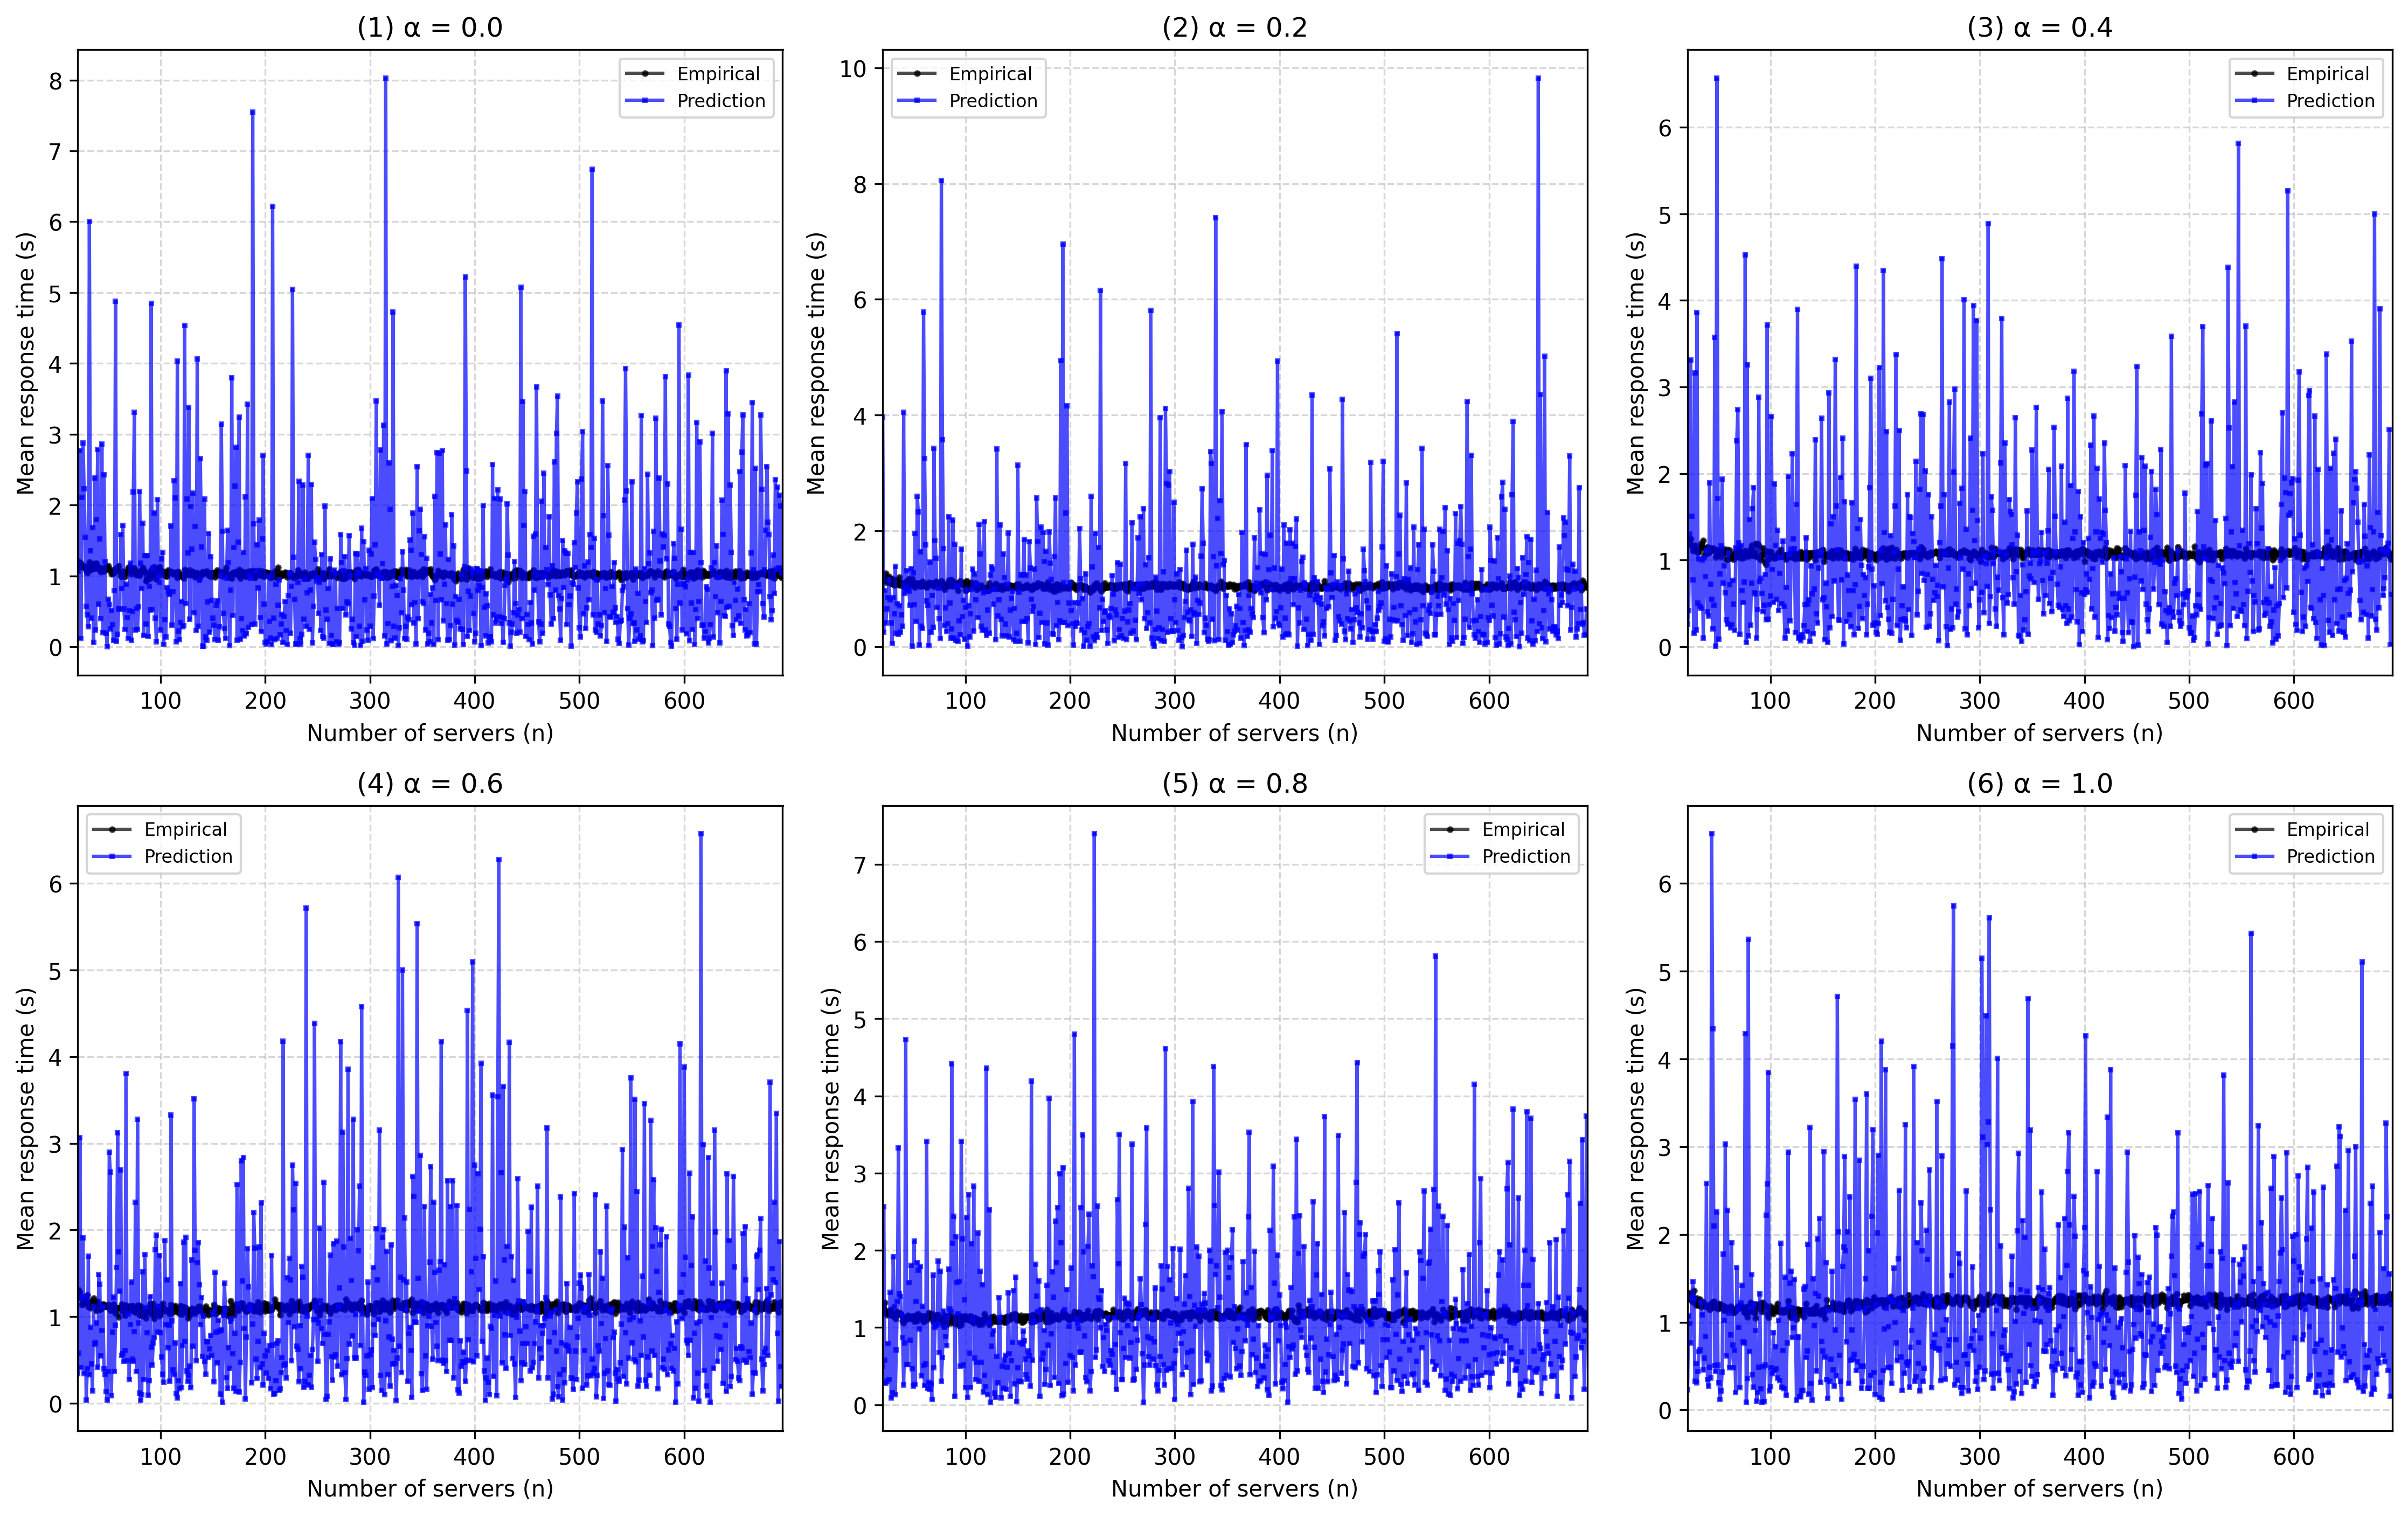
\includegraphics[height=8cm]{naive_mu_prediction.png} \\
  \caption{Аналитическое моделирование системы на основе среднего времени обслуживания измеренного в контейнерах.}
  \label{fig:naive_model_metrics}
\end{figure}

\begin{table}[htbp]
  \centering
  \caption{Сравнение производительности наивной модели в зависимости $\alpha$}
  \label{tab:naive_model_metrics}

  \renewcommand{\arraystretch}{1.2}

  \begin{tabular}{c r r r}
    \toprule
    $\alpha$         & \multicolumn{1}{c}{RMSE} & \multicolumn{1}{c}{MAE} & \multicolumn{1}{c}{MAPE (\%)} \\
    \midrule
    0,0              & 1,0909                   & 0,7821                  & 75,8992                       \\
    0,2              & 1,1204                   & 0,7725                  & 73,8104                       \\
    0,4              & 0,9573                   & 0,7093                  & 65,9469                       \\
    0,6              & 1,0069                   & 0,7382                  & 66,5865                       \\
    0,8              & 0,9388                   & 0,7013                  & 60,7633                       \\
    1,0              & 1,0028                   & 0,7644                  & 62,5456                       \\
    \midrule
    \textbf{Средний} & \textbf{1,0195}          & \textbf{0,7446}         & \textbf{67,5920}              \\
    \bottomrule
  \end{tabular}
\end{table}

\subsection{Полиномиальная регрессия для предсказания $\mu(n,\alpha,i)$}

В наших экспериментах было выявлена важность увеличения качества измерений среднего времени обслуживания комбинаций $(n, \alpha, i)$ путем фильтрации тех пар не имеющих достаточное количество данных. На рисунке \ref{fig:average_performance_metrics_vs_minimum_sample_count} можно увидеть метрики качество RMSE, MAE и MAPE в зависимости от минимального количества комбинаций. А так же количество уникальных комбинаций которые остались после фильтрации.

\begin{figure}[!htbp]
  \centering
  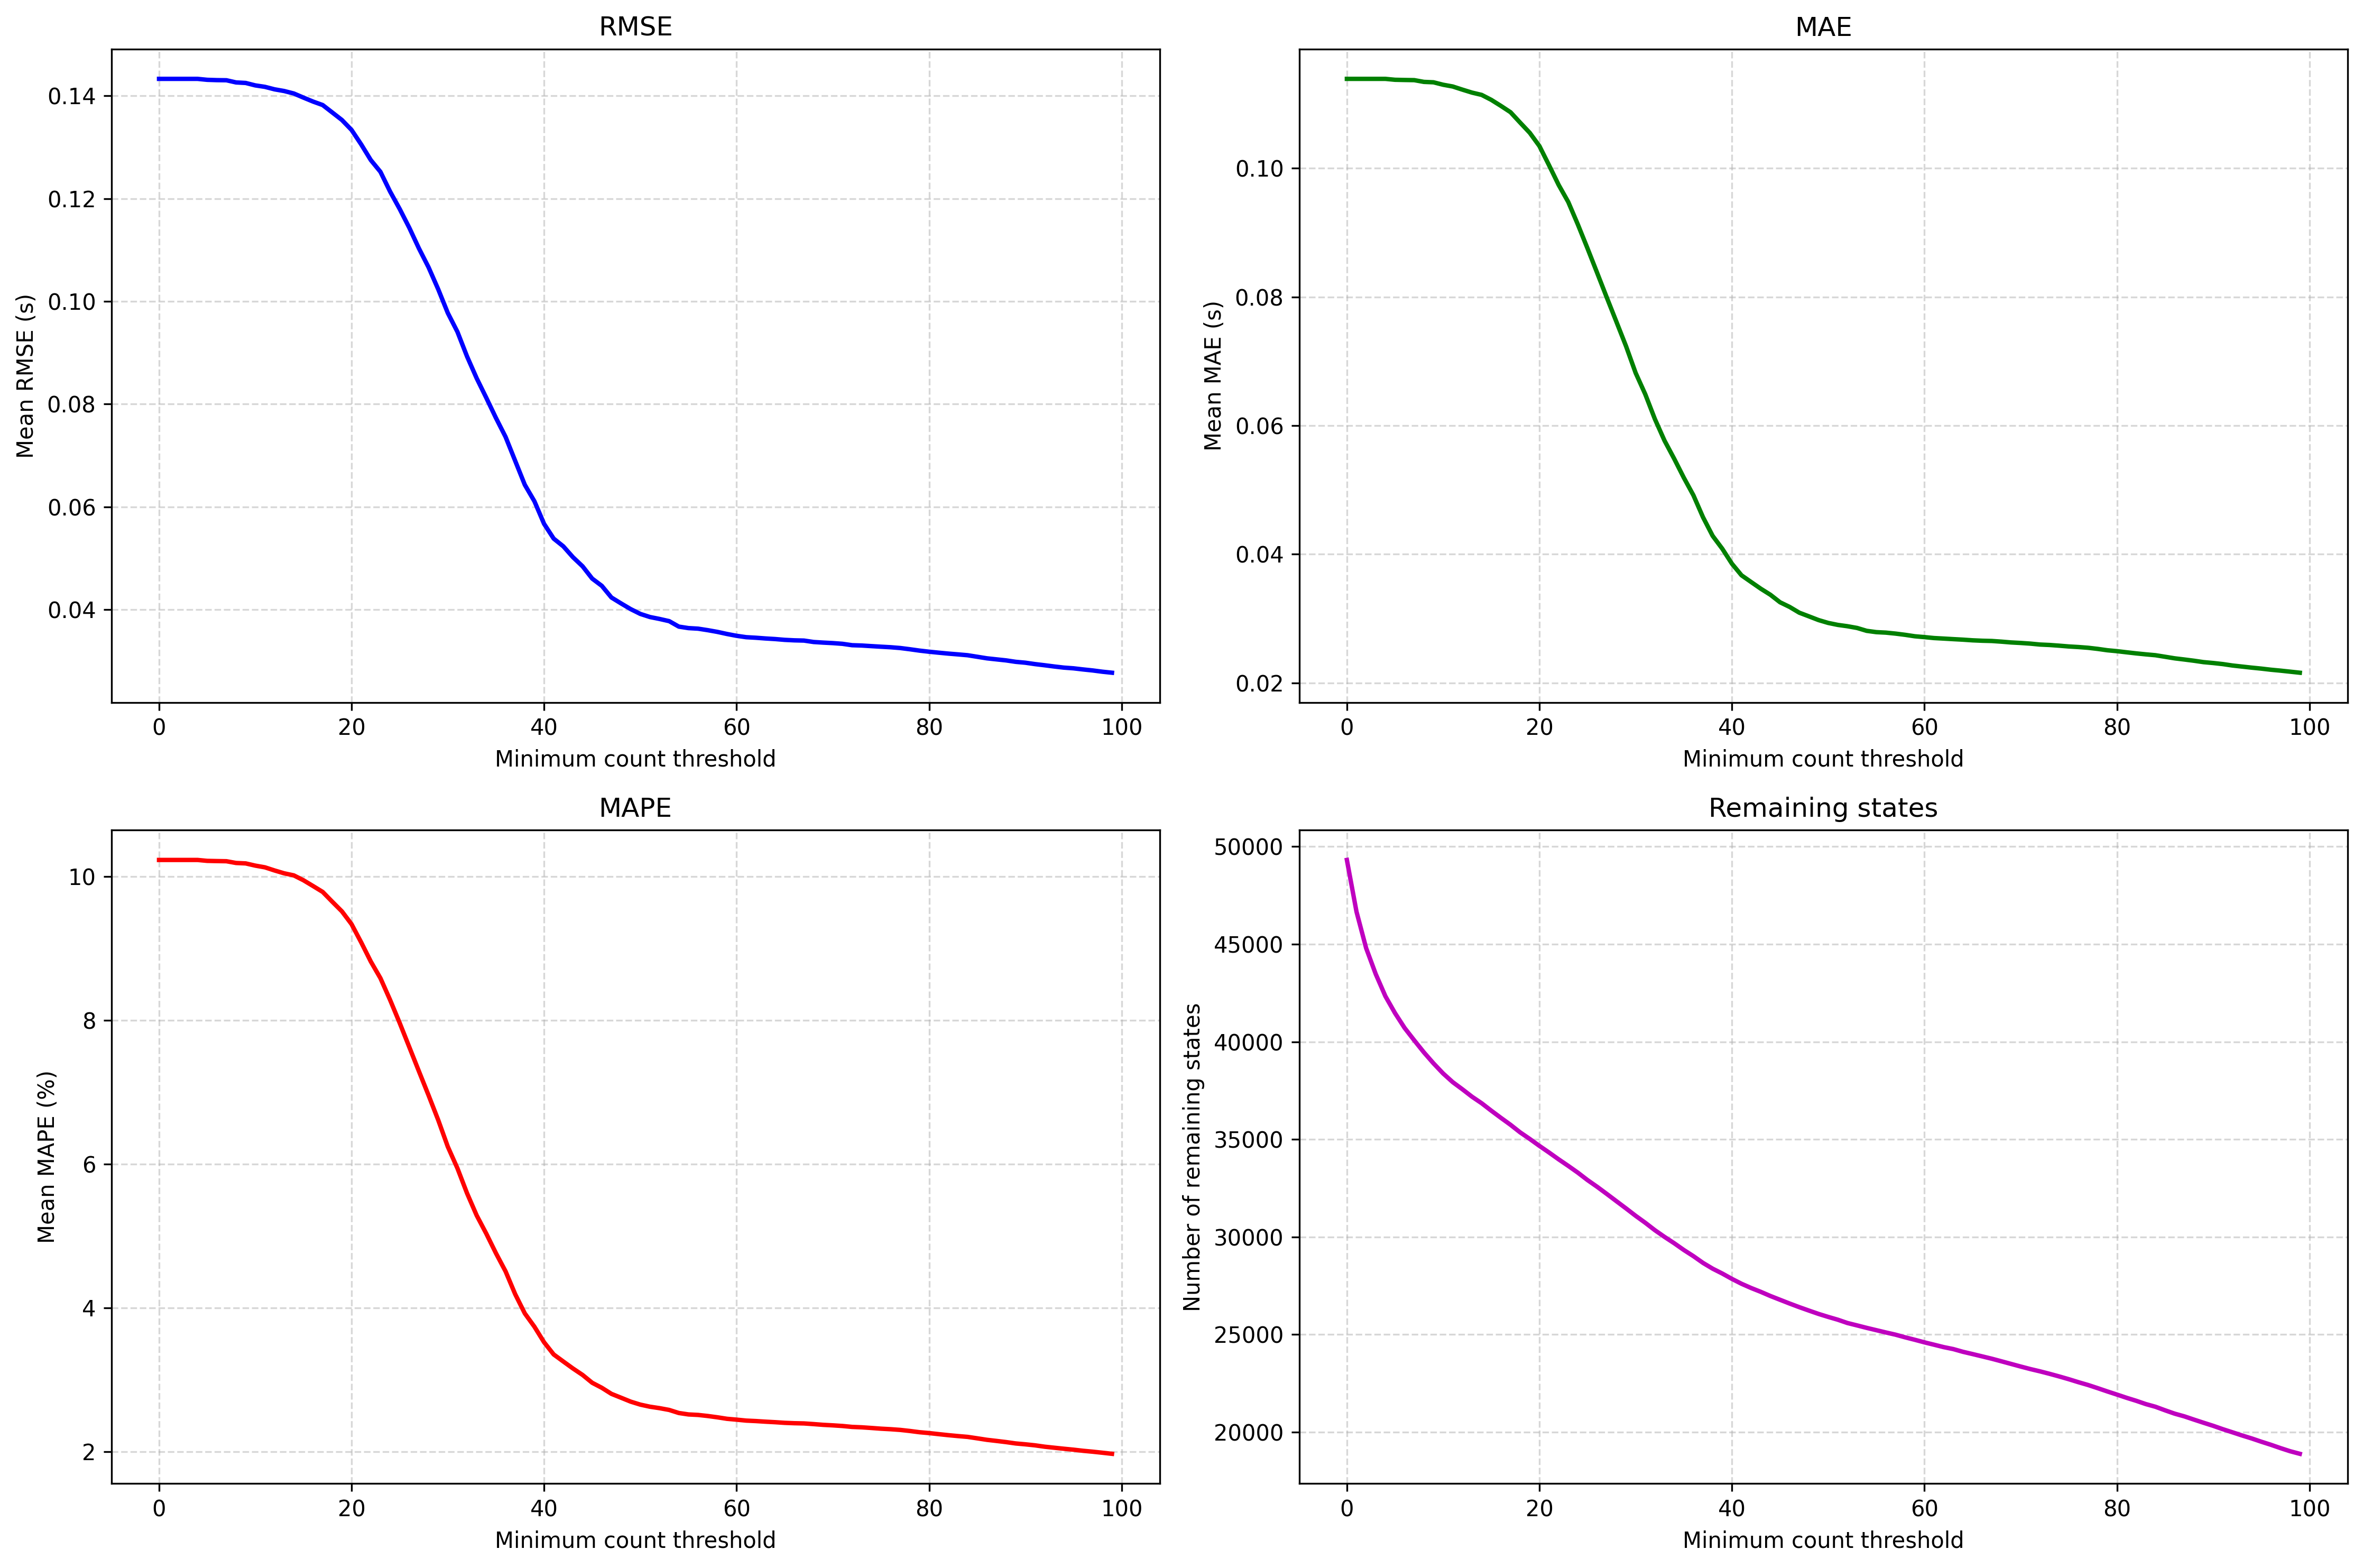
\includegraphics[height=8cm]{average_performance_metrics_vs_minimum_sample_count.png} \\
  \caption{Средние метрики производительности RMSE, MAE, MAPE (усреднённые по всем значениям $\alpha$) в зависимости от минимального количества наблюдений. Количество пар $(n, \alpha, i)$ после фильтрации.}
  \label{fig:average_performance_metrics_vs_minimum_sample_count}
\end{figure}

Сравнение различных регрессионных моделей на тестовой выборке представлено в таблице \ref{tab:model_performance_comparison}. Полиномиальная регрессия второй степени показала наилучшие результаты по всем метрикам.

\begin{table}[htbp]
  \centering
  \caption{Сравнение производительности моделей на тестовой выборке}
  \label{tab:model_performance_comparison}
  \begin{tabular}{l r r r}
    \toprule
    Model              & \multicolumn{1}{c}{RMSE} & \multicolumn{1}{c}{MAE} & \multicolumn{1}{c}{MAPE (\%)} \\
    \midrule
    Polynomial (deg=2) & 0,0536                   & 0,0424                  & 3,8295                        \\
    Decision Tree      & 0,0553                   & 0,0432                  & 3,9047                        \\
    Linear Regression  & 0,0568                   & 0,0448                  & 4,0433                        \\
    Random Forest      & 0,0593                   & 0,0466                  & 4,2176                        \\
    Polynomial (deg=3) & 0,0647                   & 0,0511                  & 4,6101                        \\
    SVR (RBF)          & 0,0854                   & 0,0691                  & 6,2781                        \\
    \bottomrule
  \end{tabular}
\end{table}

\subsection{Прогнозирование времени ответа с использованием $\mu(n,\alpha,i)$}

На рис. \ref{fig:QueuingModel_mu_alpha_i} представлены предсказания регрессионной модели (синяя кривая) и фактическое время измеренное на экспериментальном стенде (чёрная кривая) с 95\% доверительным интервалом (серая область). Средний показатель качества по всем альфам описан в таблице \ref{tab:QueuingModel_mu_alpha_i_metrics}.

\begin{figure}[!htbp]
  \centering
  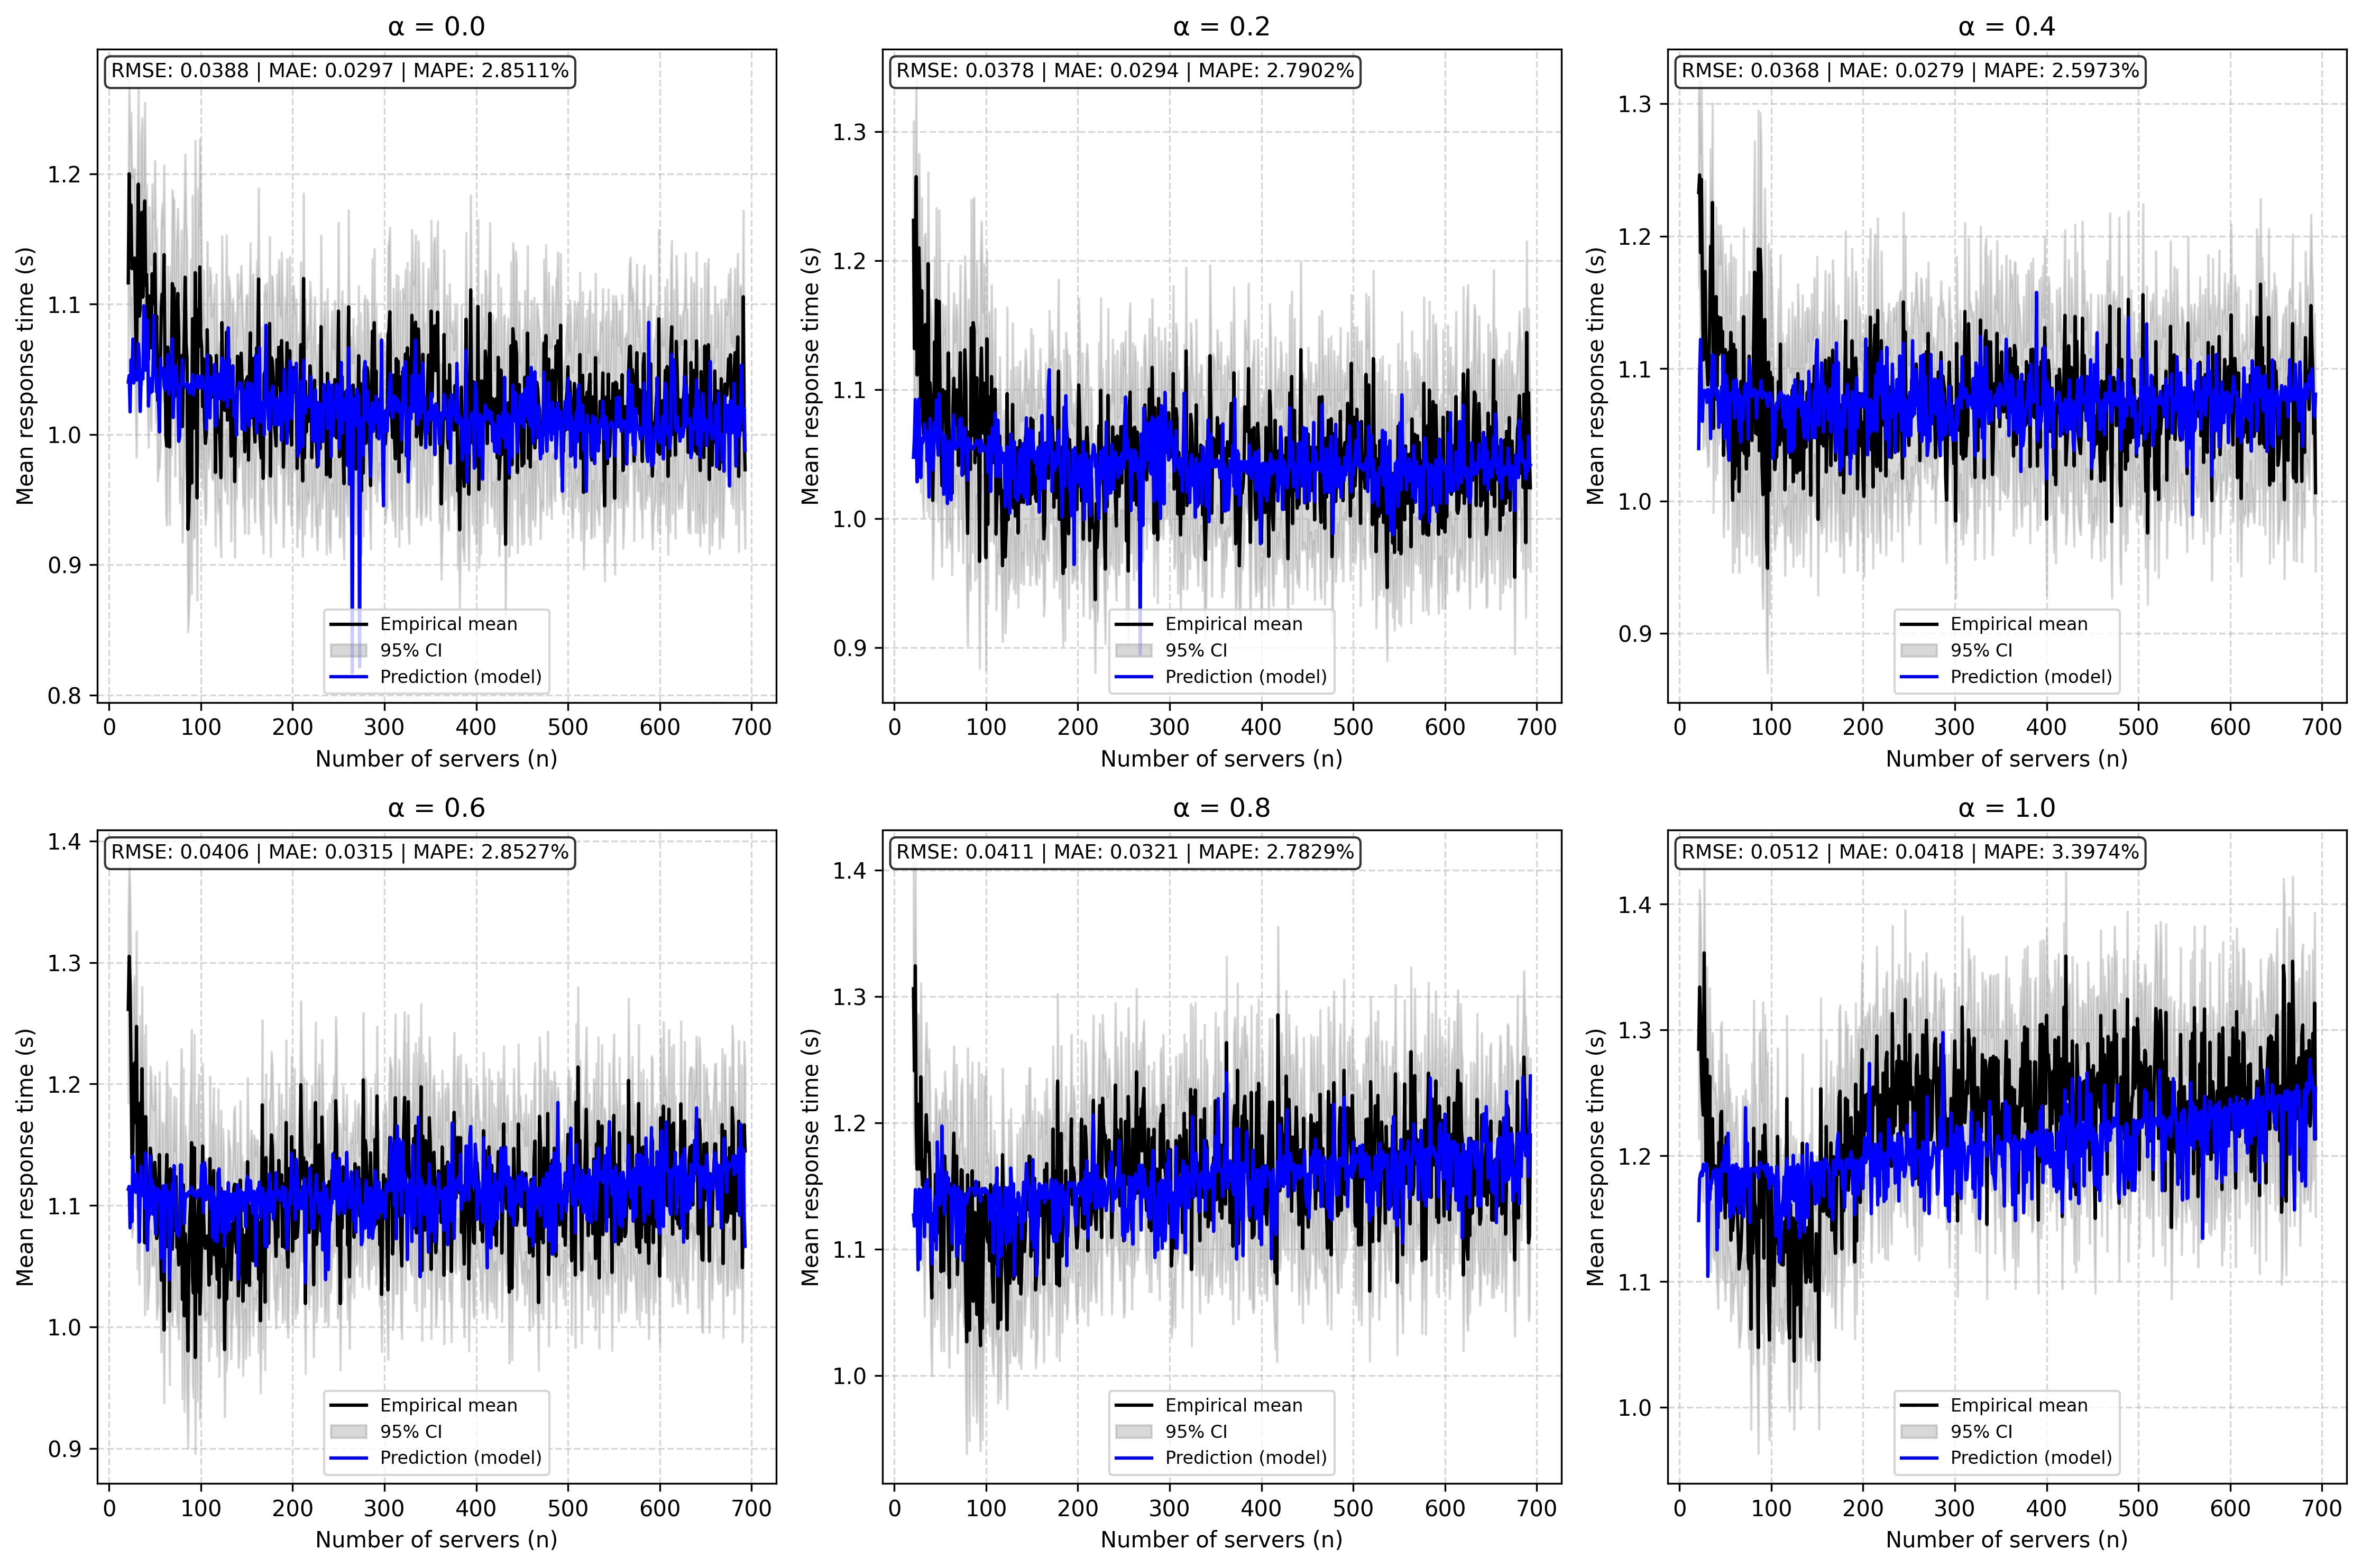
\includegraphics[height=8cm]{QueuingModel_mu_alpha_i.png} \\
  \caption{Предсказанная полиномиальной модели включающая количество запросов в системе $i$ (синим) и измеренное время обслуживания (чёрным) и доверительный интервал 95\% (серым). }
  \label{fig:QueuingModel_mu_alpha_i}
\end{figure}

\begin{table}[htbp]
  \centering
  \caption{Метрики производительности модели зависящей от состояния интенсивностью обслуживания $\mu(n,\alpha,i)$ в зависимости от $\alpha$}
  \label{tab:QueuingModel_mu_alpha_i_metrics}

  \renewcommand{\arraystretch}{1.2}

  \begin{tabular}{c r r r}
    \toprule
    $\alpha$         & \multicolumn{1}{c}{RMSE} & \multicolumn{1}{c}{MAE} & \multicolumn{1}{c}{MAPE (\%)} \\
    \midrule
    0,0              & 0,0388                   & 0,0297                  & 2,8511                        \\
    0,2              & 0,0378                   & 0,0294                  & 2,7902                        \\
    0,4              & 0,0368                   & 0,0279                  & 2,5973                        \\
    0,6              & 0,0406                   & 0,0315                  & 2,8527                        \\
    0,8              & 0,0411                   & 0,0321                  & 2,7829                        \\
    1,0              & 0,0512                   & 0,0418                  & 3,3974                        \\
    \midrule
    \textbf{Средний} & \textbf{0,0411}          & \textbf{0,0321}         & \textbf{2,8786}               \\
    \bottomrule
  \end{tabular}
\end{table}

Для сравнения, на рис. \ref{fig:QueuingModel_mu_alpha} показаны предсказания модели, не учитывающей количество запросов в системе (СМО с $\mu(n,\alpha)$, не учитывающая $i$). Качество предсказаний этой модели приведено в таблице \ref{tab:queuing_model_mu_metrics_alt}. Видно, что модель с интенсивностью $\mu(n,\alpha,i)$ даёт более точные предсказания эмпирических данных.

\begin{figure}[!htbp]
  \centering
  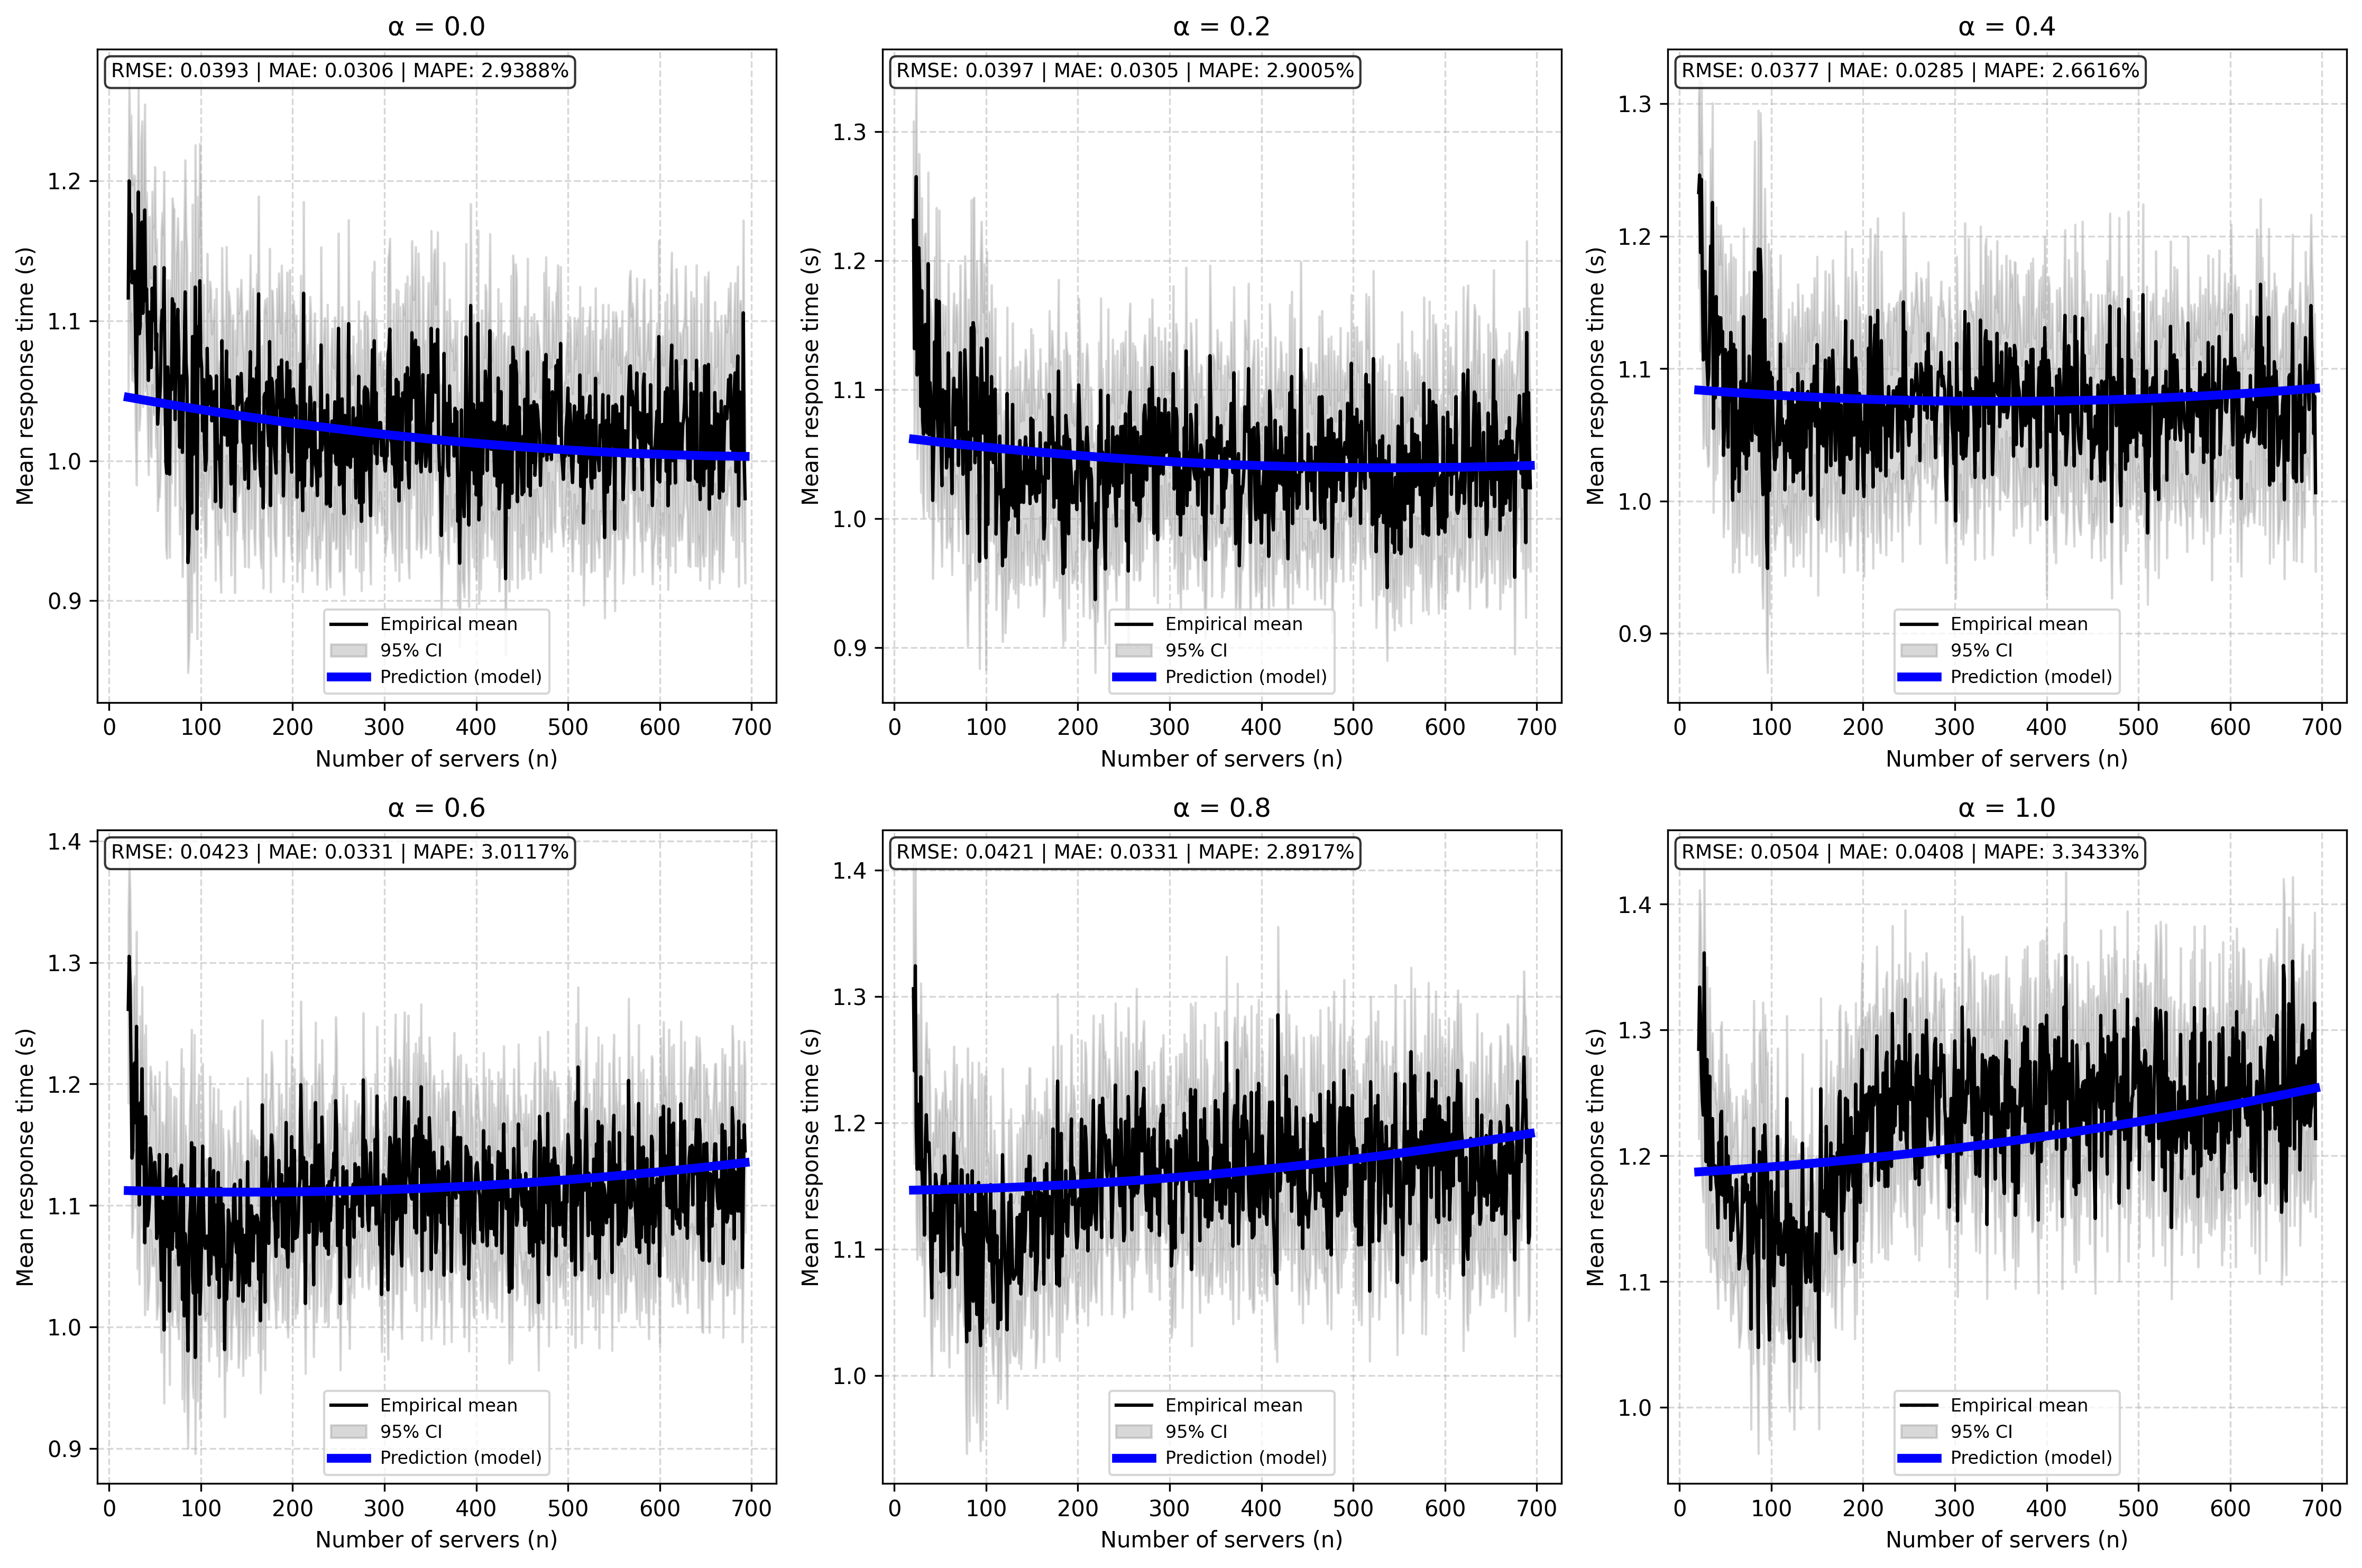
\includegraphics[height=8cm]{QueuingModel_mu_alpha.png} \\
  \caption{Предсказанная полиномиальной модели не включающей количество запросов в системе $i$ (синим) и измеренное время обслуживания (чёрным)}
  \label{fig:QueuingModel_mu_alpha}
\end{figure}

\begin{table}[htbp]
  \centering
  \caption{Метрики производительности модели с интенсивностью обслуживания $\mu(n,\alpha)$ в зависимости от $n$ и $\alpha$}
  \label{tab:queuing_model_mu_metrics_alt}

  \renewcommand{\arraystretch}{1.2}

  \begin{tabular}{c r r r}
    \toprule
    $\alpha$         & \multicolumn{1}{c}{RMSE} & \multicolumn{1}{c}{MAE} & \multicolumn{1}{c}{MAPE (\%)} \\
    \midrule
    0,0              & 0,0393                   & 0,0306                  & 2,9388                        \\
    0,2              & 0,0397                   & 0,0305                  & 2,9005                        \\
    0,4              & 0,0377                   & 0,0285                  & 2,6616                        \\
    0,6              & 0,0423                   & 0,0331                  & 3,0117                        \\
    0,8              & 0,0421                   & 0,0331                  & 2,8917                        \\
    1,0              & 0,0504                   & 0,0408                  & 3,3433                        \\
    \midrule
    \textbf{Средний} & \textbf{0,0419}          & \textbf{0,0328}         & \textbf{2,9579}               \\
    \bottomrule
  \end{tabular}
\end{table}

\subsection{Верификация имитационной модели}

Результаты валидации, представленные в таблице \ref{tab:sim_vs_empirical_and_analytical}, свидетельствуют о высокой точности имитационной модели. При сравнении с эмпирическими данными метрика MAPE для конфигурации Sim 5k составила $2,92 \pm 0,28\%$ (здесь и далее указан 95\% доверительный интервал), что подтверждает адекватность модели реальному поведению системы. RMSE для той же конфигурации равен $0,0416 \pm 0,0057$ секунды (c), а MAE $0,0325 \pm 0,0053$ (c). При этом наблюдается закономерное улучшение метрик при увеличении числа моделируемых заявок: переход от Sim 0.5k к Sim 5k снижает MAPE на $\sim12\%$ (с $3,28\%$ до $2,92\%$), что свидетельствует о сходимости имитационных оценок к истинным значениям по мере увеличения длины прогона.

Для наглядности результатов на рис. \ref{fig:analytical_vs_simulations_smooth} можно увидеть модели Sim 0.5k и Sim 2k после сглаживания используя алгоритм сглаживания Савицкого-Голея \cite{savitzky1964smoothing} из библиотеки SciPy \cite{virtanen2020scipy}. Так как Sim 5k практический совпадает с аналитической кривой, он не отображен.

Особый интерес представляет сравнение имитационной модели с аналитическим решением, которое демонстрирует ещё более высокую степень согласия. Для конфигурации Sim 5k, MAPE относительно аналитики составляет $0,50 \pm 0,5\%$, RMSE $0,0069 \pm 0,0067$ (c), MAE $0,0055 \pm 0,0054$ (c). Столь низкие значения ошибок подтверждают корректность численной реализации и алгоритмов генерации случайных величин. Узкие доверительные интервалы (порядка $1\%$ от среднего для MAPE и менее $10\%$ для RMSE и MAE) указывают на статистическую устойчивость полученных оценок и достаточное количество репликаций (пять повторений для каждой конфигурации).

\begin{table}[htbp]
  \centering
  \caption{Имитационное vs.\ Эмпирическое и Аналитическое (Средний по всем $\alpha$)}
  \label{tab:sim_vs_empirical_and_analytical}
  \begin{tabular}{lccc}
    \toprule
    Симуляция & RMSE                         & MAE                          & MAPE (\%)                    \\
    \midrule
    \multicolumn{4}{l}{\textbf{Имитационное vs Эмпирическое (Средний по всем $\alpha$)}}                   \\
    \midrule
    Sim 0.5k  & 0,0465 ($\pm$0,0406--0,0523) & 0,0364 ($\pm$0,0316--0,0412) & 3,28\% ($\pm$3,06\%--3,50\%) \\
    Sim 1k    & 0,0439 ($\pm$0,0384--0,0493) & 0,0344 ($\pm$0,0293--0,0395) & 3,09\% ($\pm$2,84\%--3,34\%) \\
    Sim 2k    & 0,0428 ($\pm$0,0373--0,0483) & 0,0335 ($\pm$0,0284--0,0385) & 3,01\% ($\pm$2,75\%--3,26\%) \\
    Sim 5k    & 0,0416 ($\pm$0,0359--0,0473) & 0,0325 ($\pm$0,0272--0,0377) & 2,92\% ($\pm$2,63\%--3,20\%) \\
    \midrule
    \multicolumn{4}{l}{\textbf{Имитационное vs Аналитическое (Средний по всем $\alpha$)}}                  \\
    \midrule
    Sim 0.5k  & 0,0218 ($\pm$0,0197--0,0238) & 0,0174 ($\pm$0,0157--0,0190) & 1,57\% ($\pm$1,50\%--1,65\%) \\
    Sim 1k    & 0,0158 ($\pm$0,0150--0,0166) & 0,0125 ($\pm$0,0119--0,0132) & 1,14\% ($\pm$1,11\%--1,18\%) \\
    Sim 2k    & 0,0110 ($\pm$0,0098--0,0122) & 0,0088 ($\pm$0,0078--0,0098) & 0,80\% ($\pm$0,76\%--0,84\%) \\
    Sim 5k    & 0,0069 ($\pm$0,0063--0,0074) & 0,0055 ($\pm$0,0050--0,0059) & 0,50\% ($\pm$0,49\%--0,51\%) \\
    \bottomrule
  \end{tabular}
\end{table}

\begin{figure}[!htbp]
  \centering
  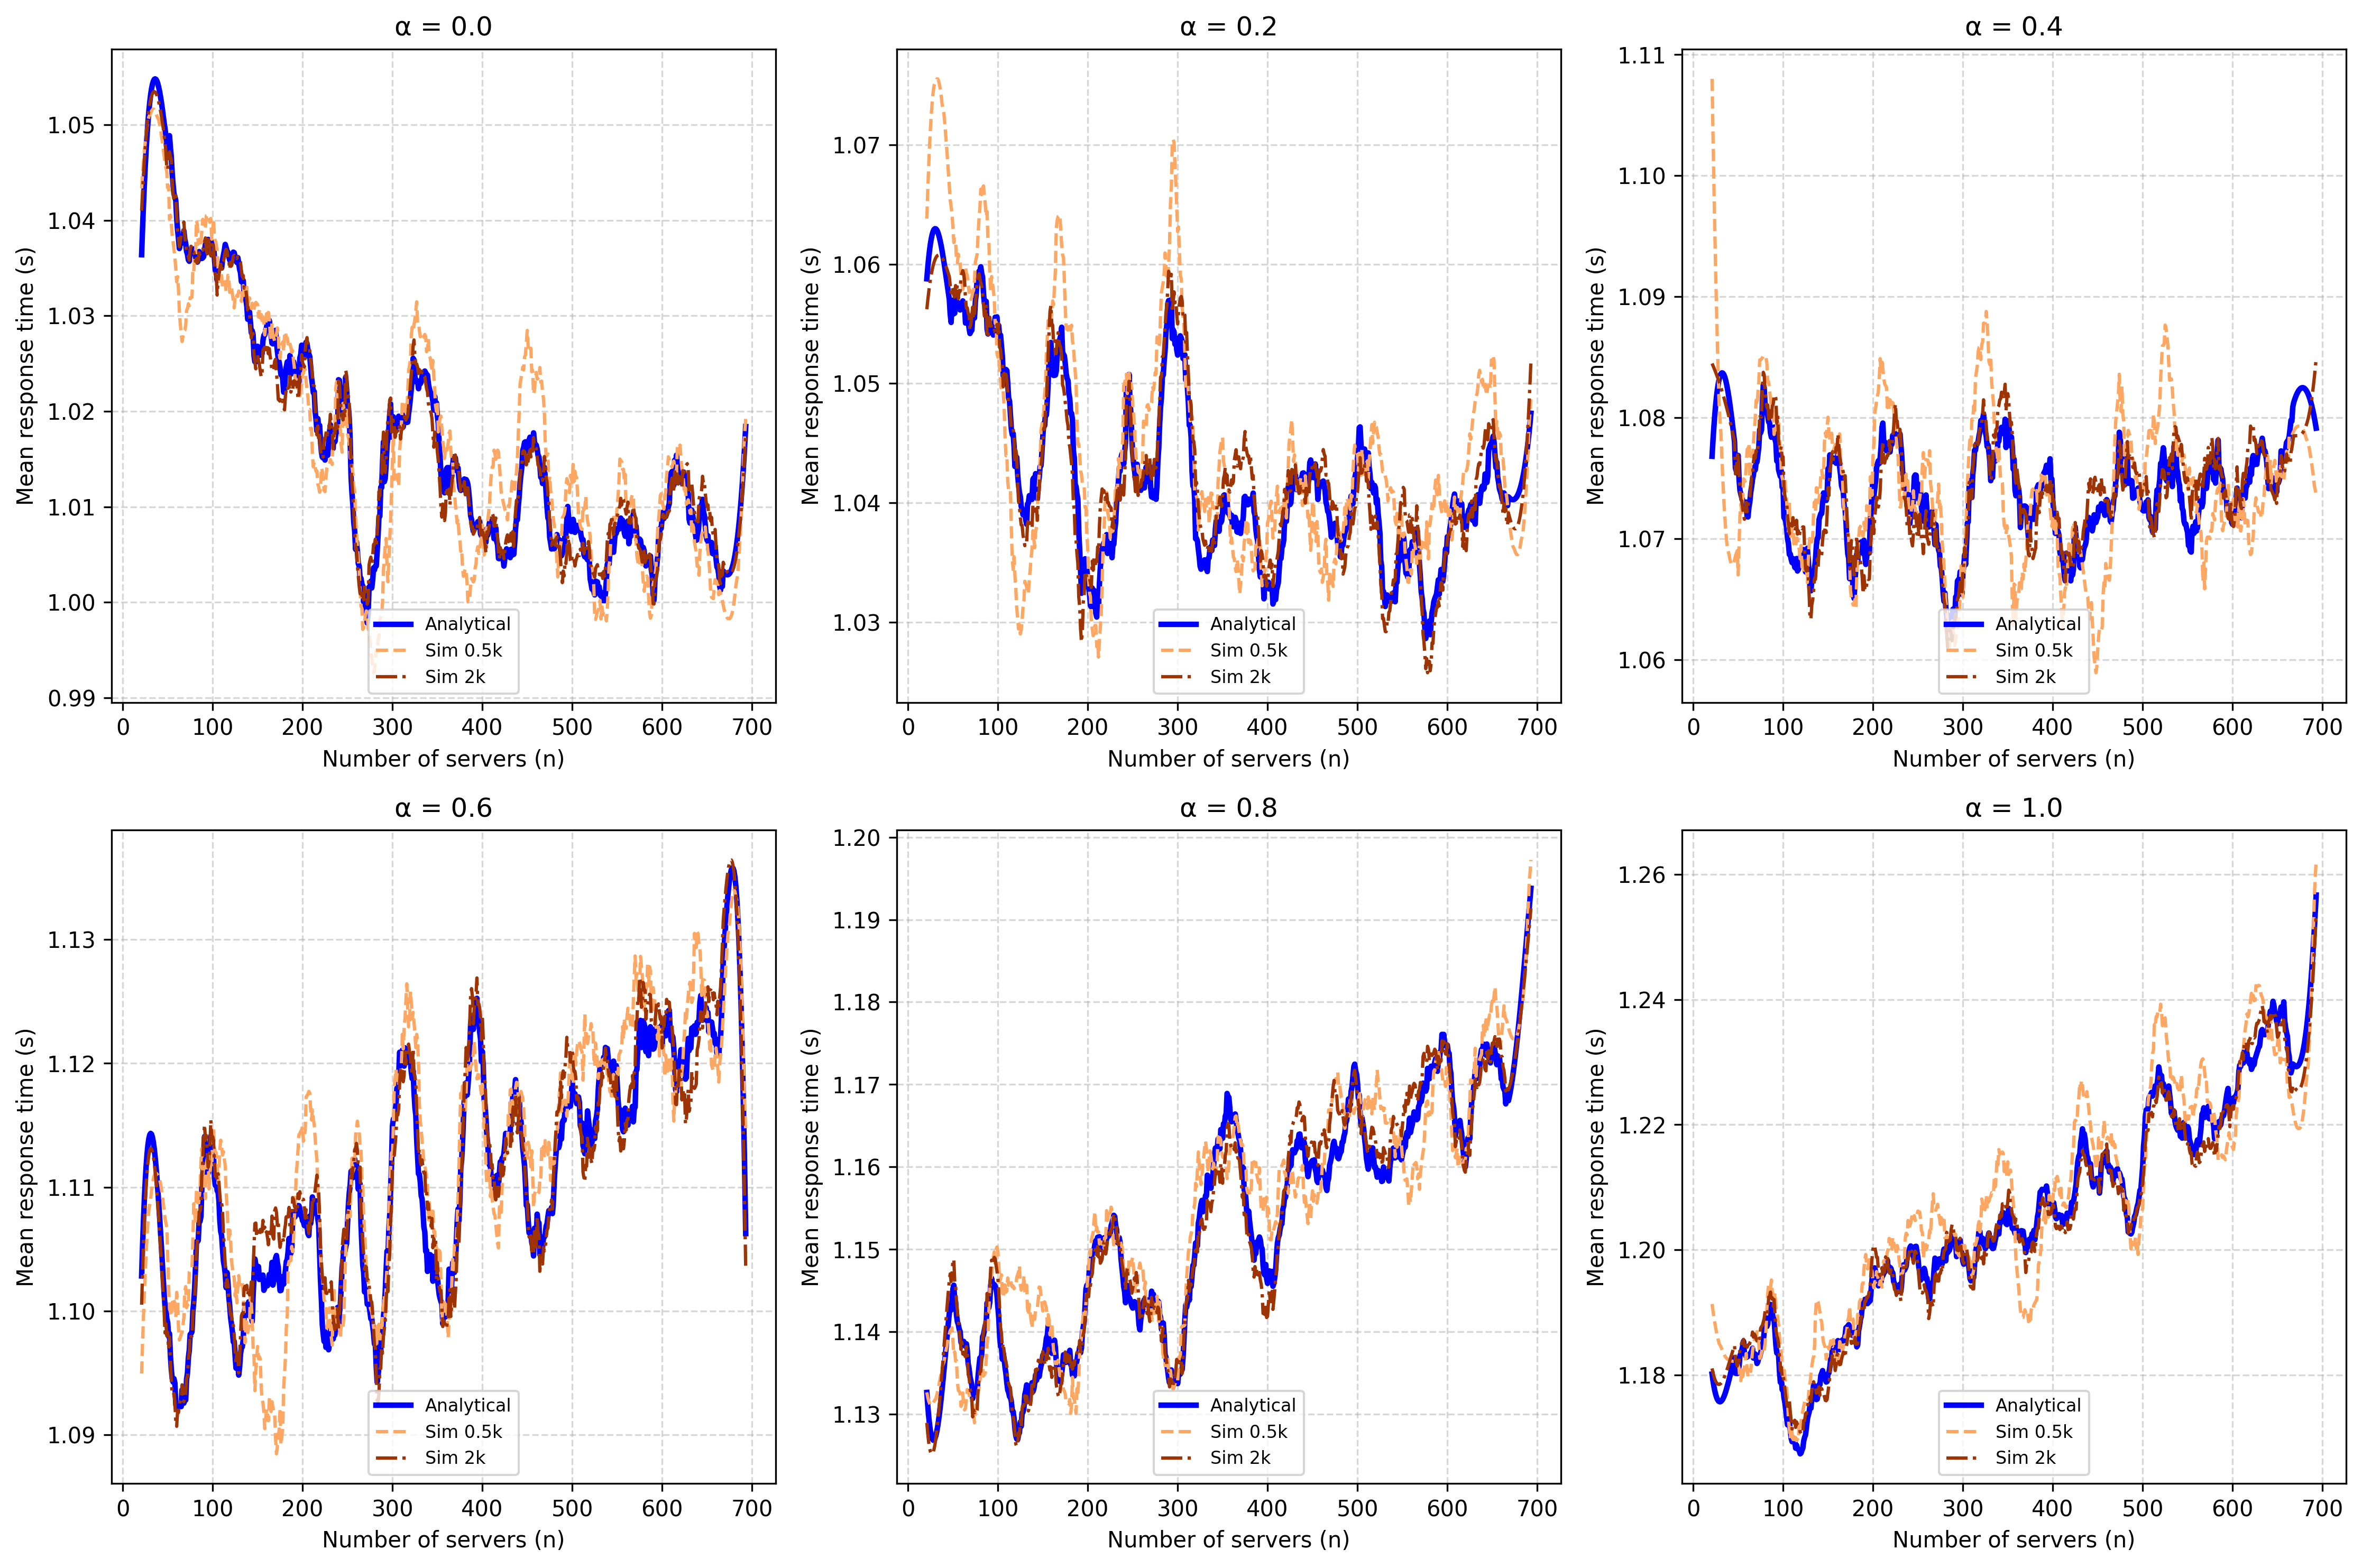
\includegraphics[height=8cm]{analytical_vs_simulations_smooth.png} \\
  \caption{Имитационное моделирование Sim 0.5k (оранжевый), Sim 2k (красный) и аналитическое вычисление (синяя сплошная). Для лучшего отображения разницы между графами, был применён алгоритм сглаживания Савицкого-Голея}
  \label{fig:analytical_vs_simulations_smooth}
\end{figure}

% ==================================================================================================
% 4. DISCUSSION
% ==================================================================================================
\section{Обсуждение}
\label{sec:discussion}

Мы построили и проверили аналитическую модель СМО. По сути, интенсивность обслуживания $\mu(n, \alpha, i)$ здесь зависит сразу от трёх факторов. Это число контейнеров, доля вычислительных задач и текущая длина очереди. Наши расчёты однозначно показывают, что игнорировать любой из этих параметров нельзя. В разделе 3 мы привели метрики. Модель с учётом $i$ выдаёт среднюю ошибку MAPE на уровне 2,88\% (таблица \ref{tab:QueuingModel_mu_alpha_i_metrics}). Упрощённый вариант, где учитываются только $n$ и $\alpha$, ошибается чуть сильнее. Там MAPE достигает 2,96\% (таблица \ref{tab:queuing_model_mu_metrics_alt}). На первый взгляд разница в сотых долях процента кажется незначительной. Но для реальной эксплуатации Kubernetes это очень много. Даже микроскопический прирост точности кардинально меняет качество автомасштабирования и соблюдение гарантий обслуживания. Заметим также, что по мере роста кластера и усложнения нагрузки этот разрыв будет только увеличиваться. Сетевые издержки и логика планировщика в крупных системах работают совершенно иначе. Фактически, чем пестрее поток запросов и непредсказуемее нагрузка, тем критичнее становится учёт текущего состояния системы.

Если сопоставить наш метод с существующими решениями, вырисовывается чёткая картина. Классические модели из \cite{pan2024performance} и \cite{kleinrock1974queueing} оперируют постоянной интенсивностью обслуживания. Это слишком грубое допущение. Наша же схема фиксирует реальную динамику, где сетевые задержки и алгоритмы балансировки напрямую привязаны к текущей загрузке. Ближайший аналог описан в \cite{van2024evaluation}. Авторы той работы тоже делают $\mu$ зависимой от числа подов и длины очереди. Причём мы пошли дальше и добавили параметр $\alpha$. Учёт доли вычислительных запросов позволяет гораздо точнее описывать гетерогенные потоки. С другой стороны, методы машинного обучения \cite{manca2023characterization, richart2025lq} выглядят крайне гибко. Однако они работают как чёрный ящик и требуют огромных размеченных выборок. В условиях дефицита телеметрии такие подходы просто неприменимы. В сущности, наша разработка удачно встраивается в нишу между строгой аналитикой и чистой эмпирикой. Мы сохраняем интерпретируемость формул, не теряя при этом в вычислительной эффективности и точности прогноза.

Разумеется, у исследования есть ряд ограничений, которые нельзя игнорировать. Пункт (а) касается базовых допущений. Мы опирались на пуассоновский входящий поток и экспоненциальное время обслуживания. Для теории массового обслуживания это классика. Но в живых кластерах хвосты распределений часто оказываются тяжелее, а сами распределения бывают мультимодальными. Пункт (б) относится к математическому аппарату. Зависимость $\mu(n, \alpha, i)$ мы оценивали через полиномиальную регрессию второй степени. В таблице \ref{tab:model_performance_comparison} видно, что она отработала лучше всех. Но это всё же аппроксимация. Глубокие нелинейные взаимодействия параметров она может сглаживать. Пункт (в) описывает аппаратную базу. Все замеры сняты на двухузловом кластере с жёстко фиксированными ресурсами. Переносить выводы на гигантские или нестандартно настроенные среды нужно с осторожностью. Наконец, пункт (г) затрагивает границы параметров. Число контейнеров $n$ не превышало 700. В реальных условиях кластеры бывают гораздо масштабнее, и экстраполяция за этот порог требует отдельной валидации. Параметр $\alpha$ мы задавали дискретно, из набора $\{0; 0,2; 0,4; 0,6; 0,8; 1\}$. Для поиска базовых закономерностей этого вполне хватило. Однако для универсального применения наверняка понадобится уже непрерывная аппроксимация.

% ==================================================================================================
% 5. CONCLUSION
% ==================================================================================================
\section{Заключение}
\label{sec:conclusion}

Предложенная модель СМО даёт инструмент для прогноза производительности кластеров Kubernetes при любой конфигурации и типе нагрузки. По сути, это позволяет обоснованно подходить к горизонтальному масштабированию, выбору числа реплик и распределению ресурсов. Особенно востребован такой прогноз в системах автомасштабирования, где время отклика нужно оценивать ещё до добавления или удаления подов. Важным аспектом нашей работы стала эмпирическая калибровка интенсивности обслуживания (раздел 3.3, формула \ref{eq:mu_eff}). Заметим, что именно она позволяет учесть все скрытые издержки конкретного развёртывания, включая сетевые задержки, особенности балансировщика и логику планировщика. Фактически, имея базовый профиль нагрузки, эту методику можно перенести на любую эксплуатационную среду.

Надёжность полученных результатов мы подтвердили перекрёстной верификацией, сопоставив натурные эксперименты с имитацией на SimPy. Для конфигурации Sim 5k расхождение между аналитикой и симуляцией не превысило 0,50\% (MAPE), что однозначно свидетельствует о корректности численной реализации. При сравнении с реальными замерами ошибка составила 2,92\% (MAPE). Причём метрики монотонно улучшались по мере увеличения длины прогона. Это прямой индикатор сходимости имитационных оценок. В сущности, проведённые проверки доказывают, что методология рабочая и применима для анализа контейнерных систем в самых разных условиях.

В планах на будущее мы видим развитие модели по нескольким векторам. Прежде всего, планируется отказ от жёсткой гипотезы об экспоненциальном времени обслуживания. Переход к гиперэкспоненциальному или фазовому распределению, а также к закону Вейбулла, откроет путь к описанию систем с куда более сложной стохастической динамикой. Ещё одно очевидное направление связано с интеграцией аналитики и методов машинного обучения. Автоматическая подстройка параметров по потоку телеметрии позволит модели адаптироваться к постепенному дрейфу характеристик кластера. Наконец, предстоит масштабировать подход на мультисервисные архитектуры, где каждый микросервис имеет собственный профиль обслуживания и уникальные требования к ресурсам.

% ##################################################################################################
\printbibliography[title={References}]
\end{document}